Como pilar fundamental de la estrategia de difusión y comercialización del proyecto, se ha diseñado una plataforma web propia accesible en la dirección: \url{https://fantastic-douhua-aab9a0.netlify.app/}. Siguiendo la filosofía de la asignatura de actuar como una ``pequeña empresa de ingeniería'', la web no solo sirve como escaparate comercial, sino también como un centro interactivo para la captación de inversores y la distribución centralizada de la documentación técnica.

\begin{figure}[H]
    \centering
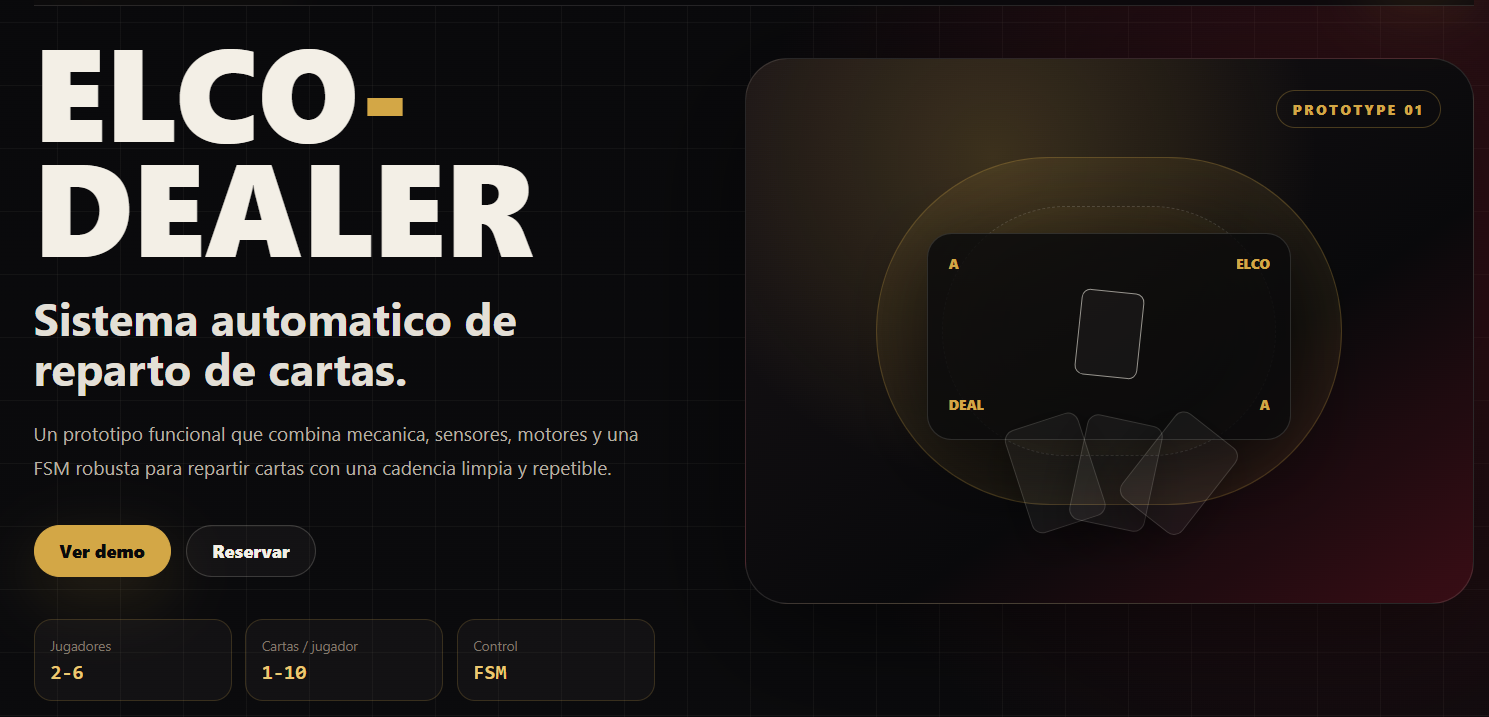
\includegraphics[width=0.85\textwidth]{inicio web (1).png}
    \caption{Interfaz principal de la web ELCO-Dealer con acceso a la Demo y reserva del prototipo.}
    \label{fig:web_hero}
\end{figure}

\subsection{Arquitectura y Contenidos de la Plataforma}

La interfaz ha sido diseñada para segmentar la información en bloques estratégicos, facilitando la comprensión del producto tanto a nivel funcional como técnico:

\begin{itemize}
    \item \textbf{Highlights y Demo:} Esta sección presenta la propuesta de valor del \textbf{ELCO-Dealer}. Incluye un video demostrativo alojado en YouTube que documenta el funcionamiento real del prototipo, su capacidad de barajado automático y el modo de uso para el cliente final (ver Figura \ref{fig:web_hero}).
    
    \item \textbf{Simulador de Reparto:} Herramienta interactiva (Figura \ref{fig:web_simulator}) que permite al usuario visualizar de forma lógica el proceso de distribución de naipes. Este simulador emula el comportamiento del software embebido en la Arduino Mega 2560, manteniendo los límites reales del prototipo (máximo 6 jugadores).
    
    \item \textbf{Engineering (Arquitectura de Software):} Se detalla el diseño orientado a la robustez (Figura \ref{fig:web_arquitectura}), destacando el uso de una \textbf{Máquina de Estados Finitos (FSM)} para gestionar la lógica de control. La web explica cómo el sistema evita bloqueos mediante la implementación de prioridades de eventos, \textit{timeouts} y transiciones claras sin acceso directo a pines para asegurar la portabilidad del código. 
    
    \item \textbf{Hardware y Sensórica:} Bloque técnico que describe la integración de los componentes clave detallados en el listado de materiales (BOM). Se resalta el uso de los drivers \textbf{L298N} para el control de potencia \cite{l298n_st}, el sensor de efecto Hall \textbf{A3144} para la autocalibración de 0 grados y los sensores infrarrojos \textbf{TCRT5000} para la detección de cartas por flancos.
    
    \item \textbf{User Interface (UI):} Detalla el subsistema de configuración. El usuario puede definir interactivamente el número de jugadores y el modo de reparto a través de la pantalla y botonera integradas.
\end{itemize}

\begin{figure}[H]
    \centering
    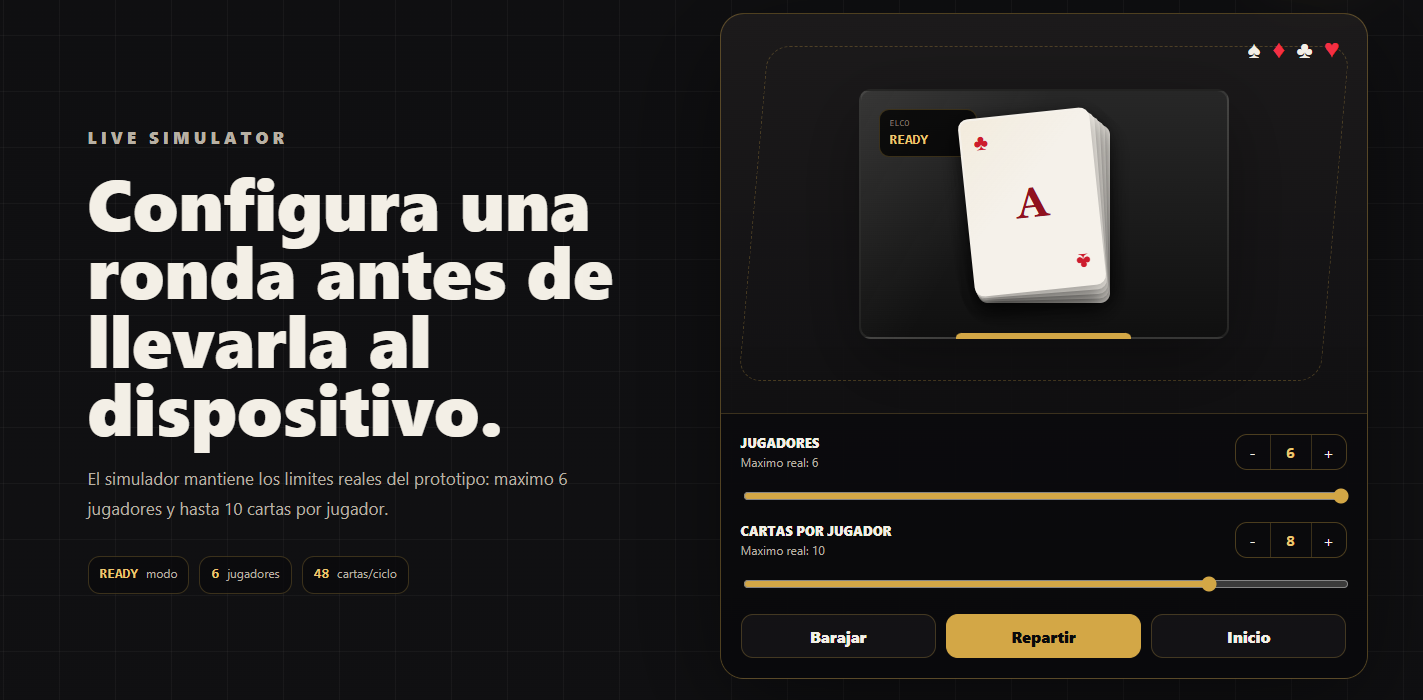
\includegraphics[width=0.85\textwidth]{web simulador.png}
    \caption{Detalle del simulador lógico de barajado y reparto integrado en la plataforma.}
    \label{fig:web_simulator}
\end{figure}

\begin{figure}[H]
    \centering
    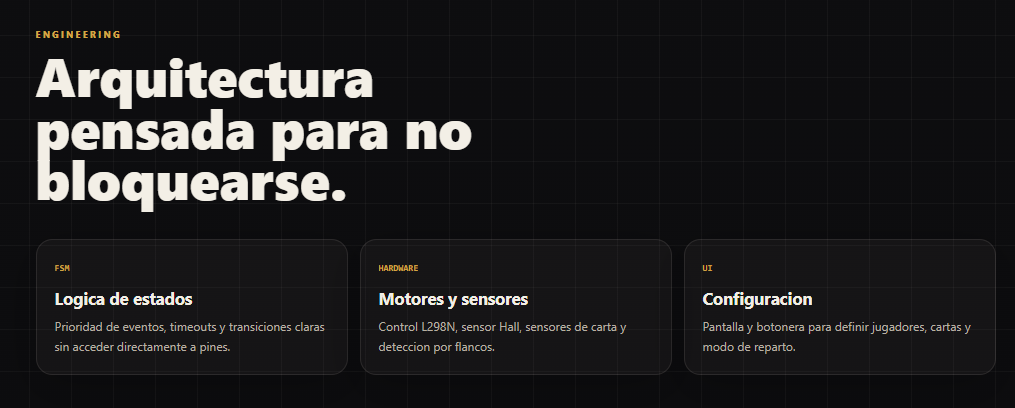
\includegraphics[width=0.85\textwidth]{web arquitectura.png}
    \caption{Detalle de la FSM, el hardware y la UI del prototipo.}
    \label{fig:web_arquitectura}
\end{figure}

\subsection{Estrategia de Captación: Wishlist y Reserva}

Siguiendo un enfoque honesto de lanzamiento de producto bajo el contexto de un proyecto de ingeniería universitaria, la web incluye una sección de reserva (Figura \ref{fig:web_wishlist}). Esta funcionalidad permite registrar el interés de posibles clientes y construir un \textit{storytelling} creíble alrededor del prototipo, alineándose con la viabilidad económica planteada en la memoria del proyecto.

\begin{figure}[H]
    \centering
    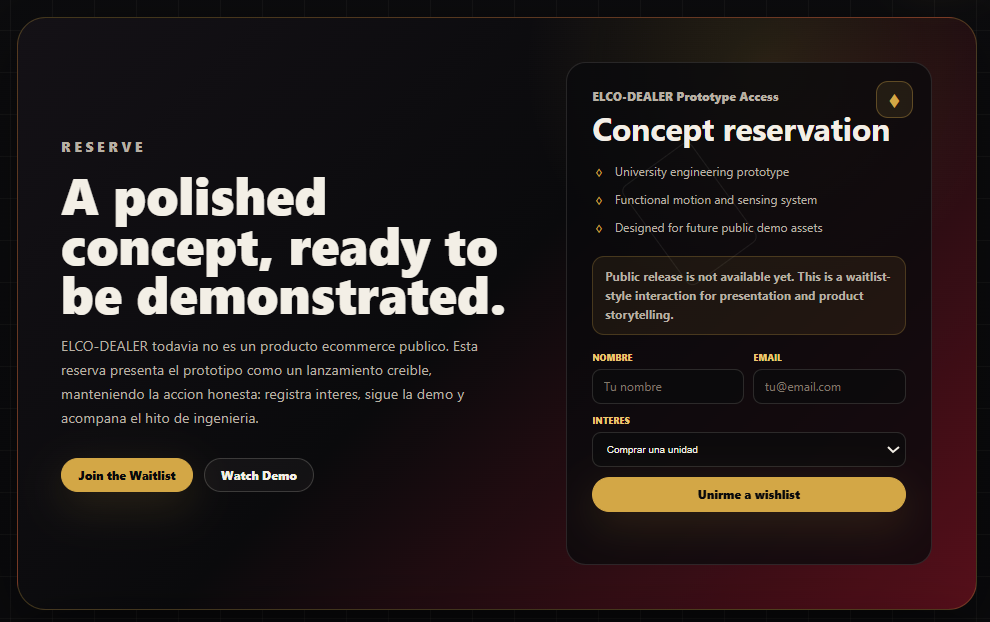
\includegraphics[width=0.85\textwidth]{wishlist.png}
    \caption{Formulario de reserva y wishlist integrado en la plataforma web.}
    \label{fig:web_wishlist}
\end{figure}


\subsection{Integración con la Filosofía Open Source}

En cumplimiento con los requisitos de documentación pública de la asignatura, el pie de página de todas las secciones incluye enlaces directos a los resultados publicados en redes de distribución técnica:
\begin{itemize}
    \item \textbf{GitHub:} Repositorio con el código fuente completo y pruebas de módulos \cite{github_link}.
    \item \textbf{Instructables:} Guía paso a paso para la replicación del proyecto por parte de la comunidad \cite{instructables_link}.
\end{itemize}










